% Emacs, this is -*- latex -*-!
\chapter{Differentiation in practice}
\label{sec:applying}

In practice, successful incrementalization requires both
correctness and performance of the derivatives. Correctness of
derivatives is guaranteed by the theoretical development the
previous sections, together with the interface for
differentiation and proof plugins, whereas performance of
derivatives has to come from careful design and implementation of
differentiation plugins.

\section{The role of differentiation plugins}
\label{ssec:methodology}
Users of our approach need to
%
(1) choose which base types and primitives they need,
%
(2) implement suitable differentiation plugins for these base
types and primitives,
%
(3) rewrite (relevant parts of) their programs in terms of these primitives and
%
(4) arrange for their program to be called on changes instead of
updated inputs.

As discussed in \cref{sec:informal-derive}, differentiation
supports abstraction, application and variables, but since
computation on base types is performed by primitives for those
types, efficient derivatives for primitives are essential for
good performance.

To make such derivatives efficient, change
types must also have efficient implementations, and allow
describing precisely what changed. The efficient derivative of
$\Term{sum}$ in \cref{sec:intro} is possible only if bag changes
can describe deletions and insertions, and integer changes can
describe additive differences.

For many conceivable base types, we do not have to design the
differentiation plugins from scratch. Instead, we can reuse the
large body of existing research on incrementalization in
first-order and domain-specific settings. For instance, we reuse
the approach from \citet{GlucheGrust97Incr} to support incremental
bags and maps. By wrapping a
domain-specific incrementalization result in a differentiation
plugin, we adapt it to be usable in the context of a higher-order
and general-purpose programming language, and in interaction with
other differentiation plugins for the other base types of that
language.

% Emacs, this is -*- latex -*-!
\begin{figure*}
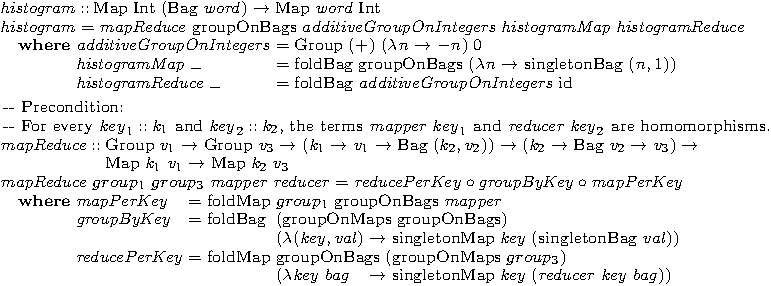
\includegraphics{pldi14/fig-mapReduce.pdf}
\caption{The $\Gl$-term $\HISTOGRAM$ with Haskell-like syntactic
  sugar. $\Term{additiveGroupOnIntegers}$ is the abelian group induced on
  integers by addition $(\mathbb{Z}, +, 0, -)$.}
\label{fig:case-study-pseudocode}
\end{figure*}

  
For base types with no known incrementalization strategy,
the precise interfaces for differentiation and
proof plugins can guide the implementation effort. These
interfaces could also from the basis for a library of
differentiation plugins that work well together.

Rewriting whole programs in our language would be an excessive
requirements. Instead, we embed our object language as an EDSL in
some more expressive meta-language (Scala in our case study), so
that embedded programs are reified. The embedded language can be
made to resemble the metalanguage~\citep{rompf2010lightweight}.
To incrementalize a part of a computation, we write it in our
embedded object language, invoke $\DERIVE$ on the embedded
program, optionally optimize the resulting programs and finally
invoke them. The metalanguage also acts as a macro system for the
object language, as usual. This allows us to simulate polymorphic
collections such as $\Bag*[\Gi]$ even though the object language is
simply-typed; technically, our plugin exposes a family of base
types to the object language.

\pg{Explain how we construct changes? The metalanguage can then
  construct changes in different ways?}



  \begin{oldSec}
\section{Methodology}
\label{ssec:methodology}


\begin{itemize}
\item We identify (classes of) base types which are relevant for
  our application, together with any relevant equational properties.
\item We define change representations for these base
  types.
\pg{Here we should give some criteria, if we can.}
\pg{For instance, restrictions on change structures which are
  erased become additional invariant for the change types.}
\pg{For instance, we should
  discuss the point of this paragraph:
``Furthermore, derivatives need to inspect the intensional
structure of changes, which are typically small, without applying
them to their base value, which is typically big. The interface
to do this depends on the specific change structure, hence we
specify no generic operation to allow this.''
}
\item We design for each (class of) base type a relevant set of
  primitives.  Where
  useful, we provide optimized derivatives for such primitives.
  We try to define primitives which capture
  incrementalizable computation skeletons; if such primitives are
  not general enough, we can add additional primitives which are
  more general but whose derivatives are less efficient.
\item We transform target programs to use our primitives.
\end{itemize}

\pg{I need self-maintainability and predicting nil changes here
  to discuss the example. So maybe the example should just be
  part of the case study.}
For instance, \citet{GlucheGrust97Incr} incrementalize bags for a
first-order language. By adapting/extending those techniques, we
can integrate bags into our higher-order language.

\pg{We should say dictionary, not map, for reduced ambiguity with the map operation.}
Using similar techniques, we also implemented support for the
operation on maps needed in our case study.

\pg{This section should also explain where changes come from.}
\end{oldSec}



\section{Predicting nil changes}
Handling changes to all inputs can induce excessive overhead in incremental
programs~\citep{Acar09}. It is also often
unnecessary; for instance, the function argument of $\Term{fold}$ in 
\cref{sec:intro} does not change since it is a closed subterm of the program, so
$\Term{fold}$ will receive a nil change for it.
A (conservative) static analysis can detect changes that are guaranteed to be nil at runtime. 
We can then specialize derivatives that receive this change, so that they need not
inspect the change at runtime.

For our case study, we have implemented a simple static analysis which
detects and propagates information about closed terms. The analysis is not interesting and 
we omit details for lack of space.



% Emacs, this is -*- latex -*-!

\subsection{Self-maintainability}
\label{sec:performance-cons}
\label{ssec:self-maint}

\begin{oldSec}
On its own, deriving $\Gl$-abstractions, applications and
variables (\cref{fig:correctness:derive}) does not improve performance.
It only relates the computations embodied in the primitives in
an incremental and higher-order setting, and provides a method to
generalize the vast quantity of research on first-order incremental
computation in the field of databases.
Our first approach toward performance gain is based on the idea of \emph{self-maintainable uses of primitives};
other approaches are certainly feasible. We did not formalize the
optimizations or prove them correct.
\end{oldSec}

In databases, a self-maintainable view~\citep{Gupta99MMV} is a function that can
update its result from input changes alone, without looking at
the actual input. By analogy, we call a derivative
\emph{self-maintainable} if it uses no
base parameters, only their changes. Self-maintainable derivatives
describe efficient incremental computations: since they do not
use their base input, their running time does not have to depend on the input
size.

\begin{examples}
$\Derive{\MERGE} = \Lam {x\; \D x\; y \; \D y}{\Merge{\D x}{\D y}}$
is self-maintainable with the
change structure $\ChangeStruct{\Bag{S}}$ described in
\cref{ssec:change-structures}, because it does not use the base
inputs $x$ and $y$.
Other derivatives are self-maintainable only in certain contexts.
The derivative of element-wise function application
$\App*{\App\MAP f}{\mathit{xs}}$ ignores the original
value of the bag $\mathit{xs}$ if the changes to
%
$f$ are always nil, because the underlying primitive $\FOLDBAG$
is self-maintainable in this case (as discussed in next section).
%
We take advantage of this by implementing a specialized
derivative for $\FOLDBAG$.

We have seen in \cref{ssec:differentiation} that $\Derivative$
needlessly recomputes $\Merge\Xs\Ys$. However, the result is a
base input to $\FOLD'$.
%
In next section, we'll replace $\FOLD'$ by a self-maintainable
derivative (based again on $\FOLDBAG$) and will avoid this
recomputation.
\end{examples}

%% Rationale for previous statement. Too complicated; left out.
%deriving a closed term without primitives yields a term that is
%self-maintainable whenever its higher-order arguments receive
%self-maintainable changes.
%The default rule $\Derive{c} = \Diff c c$ does not yield
%self-maintainable derivatives, because $\DIFF$ and $\APPLY$ use
%the input~$x$ in a significant way (\cref{fig:diff-apply}).
%However,

To conservatively predict whether a derivative is going to be
self-maintainable (and thus efficient), one can inspect whether
the program restricts itself to (conditionally) self-maintainable
primitives, like $\MERGE$ (always) or $\MAP \APP f$ (only if $\D
f$ is nil, which is guaranteed when $f$ is a closed term).

%% From the author response.
%It is possible to give a conservative approximation of whether a program's derivative is self-maintainable:
%If the original program only uses primitives with fully
%self-maintainable derivatives, the derivative of the program will
%be self-maintainable, too. We can syntactically approximate full
%self-maintainability of a primitive by checking whether the code
%of its derivative uses the $x$ variable (in addition to $\D x$) \pg{bind x! What about multiple arguments?}. For
%instance, the derivative of $\MERGE$ uses only $\D x$ and $\D y$, never $x$
%or $y$, and is hence fully self-maintainable. The derivative of
%$\FOLDBAG$ uses both $f$ and $\D f$; it is only self-maintainable
%sometimes (when df is the nil change).

\begin{oldSec}
Sometimes we can safely replace the derivative of a primitive by
a self-maintainable term, in which case we call it a
\emph{self-maintainable use of a primitive.}
Terms have self-maintainable derivatives if they use
primitives in a self-maintainable manner.

\pg{As Klaus points out, this is not true until we fix the set of
  changes - discussed in \#265. So we should specify the set of
  changes, or use a different example. We should also motivate
  it.}
%
\pg{Agreed: Convert to bags and to our running example, using foldBag.}
To illustrate, suppose $\MAP$ is a primitive of sets of
integers,
and changes to sets consist of insertions and deletions only.
The term
\[
\Lam x {\MapT {\Lam*n {n + 1}} x}
\]
contains a self-maintainable use of $\MAP$, because any change to
the input set~$x$, say $\{\App\INSERT5, \App\DELETE7\}$, can be
converted to an output change, say $\{\App\INSERT6,
\App\DELETE8\}$, without looking at $x$ itself. The use of $\MAP$
in the following term is not self-maintainable:
\[
\Lam x {\MapT {\Lam*n {n + \Sum* x}} x}.
\]
Even one insertion to the input set~$x$ generates a sweeping
change over all elements of the output set that is impossible to
express in terms of insertions and deletions without knowledge of $x$.

\pg{Before this, show that some of our primitives are
  self-maintainable, and some are self-maintainable if some
  inputs are nil.}
Our prototype optimization framework proceeds in two steps.
\begin{enumerate}
\item A static analysis identifies when changes are guaranteed to be nil.
\item During the differentiation transformation, $\DERIVE$
selects an appropriate self-maintainable function whenever possible,
considering the results of the static analysis.
\end{enumerate}
Due to space constraint, we cannot go into details of those
steps.
%
\yc{link to code}
%
\end{oldSec}

To avoid recomputing base arguments for self-maintainable derivatives
(which never need them), we
currently employ lazy evaluation.  Since we could use standard techniques for dead-code
elimination~\citep{Appel97} instead, laziness is not central to our
approach.

A significant restriction is that not-self-maintainable derivatives can require expensive computations to supply their base
arguments, which can be expensive to compute. Since they are also
computed while running the base program, one could reuse the previously
computed value through memoization or extensions of static
caching (as discussed in \cref{ssec:staticmemo}). We leave implementing these optimizations for future work. As a consequence,
our current implementation delivers good results only if
most derivatives are self-maintainable.

\begin{oldSec} % ID=Appel97
\pg{Do not remove without universal agreement. I don't think the paper can avoid discussing this aspect. }
One important issue is left. In a call-by-value
implementation of lambda calculus, running the program
\[
\Derive{\App{s}{t}} = \App{\App{\Derive{s}}{t}}{\Derive{t}}
\]
computes $t$
again, even though it was computed in the base program, thus
leading to wasteful repeated computation.
However, we claim this is a simpler problem to solve.
Three possibilities arise:
\begin{enumerate}
\item $t$ is very cheap to compute (for instance, it is a
  literal), so the problem does not occur.
\item $t$ is passed to a function which does not use it, hence
  we can avoid computing it using separate optimization steps, by
  executing the derivative with a lazy semantics (as done in our
  benchmarks) or (we expect) by using known techniques for
  interprocedural dead-code elimination~\citep{Appel97}.
\item Otherwise, since the term $t$
  was already computed while running the base
  program, we can save its value for use in the derivative.
  Approaches to
  implement this include memoization~\pg{cite} and extensions of
  static caching (as discussed in Sec.~\ref{sec:rw}).
  We leave investigating the different
  approaches to future work.
\end{enumerate}
\end{oldSec}

\begin{oldSec} % ID=Gupta99MMV
We next analyze when $t$ is going to be unused.
Inspecting the definition of $\DERIVE$ shows that only derivatives of (functions
containing) primitives can use $t$. For instance,
$\Derive{\Lam{x}{x}} = \Lam{x}{\Lam{\D x}{\D x}}$ does not use its
base input $x$, because $\Derive{x} = \D x$.
\pg{Make this more tentative. Remove 'prove'.}
It's easy to prove
by induction that if derivatives of primitives appearing in $s$
do not use their base input, neither does $s$.\footnote{Function
  changes coming from outside the program are not covered by this
  proof and are possible counterexamples.}

We term primitives whose derivative does not use their base input
self-maintainable, by analogy with the database concept of
self-maintainable views~\citep{Gupta99MMV}. \ko{Give example of 
self-maintainable and non-self-maintainable primitive}. 
We then extend this to programs: a
closed program is self-maintainable if its result does not depend
on base inputs or base intermediate results.
%
For programs which do not depend on functions as parameters (and
whose derivatives hence do not have function changes as
parameters), it should be straightforward to prove that being
self-maintainable is equivalent to only using self-maintainable
primitives.

Hence, we can argue informally that if a program only uses
self-maintainable primitives, its derivative will not recompute
base intermediate results (except if they are computed for
unrelated reasons). In our case study (Sec.~\ref{sec:eval}),
such derivatives are already
extremely efficient.

\pg{This should be somehow better integrated in the rest of the section.}
\end{oldSec}


\section{Case study}
\label{sec:plugins}
\pg{change naming for derivatives, they're dfold not fold' now.}

We perform a case study on a nontrivial realistic program to
demonstrate that \ILC\ can speed it up.
We take the MapReduce-based skeleton of the
word-count example~\citep{Lammel07}. We define a
suitable differentiation plugin, adapt the program to use it and show
that incremental computation is faster than recomputation.
%
We designed and implemented the differentiation plugin 
following the requirements of the corresponding proof plugin,
even though we did not formalize
the proof plugin (e.g. in Agda).
For lack of space, we focus on base types
which are crucial for our example and its performance, that is,
collections.
%
The plugin also implements tuples, tagged unions, Booleans and
integers with the usual introduction and elimination forms, with
few optimizations for their derivatives.

$\WORDCOUNT$ takes a map
from document IDs to documents and produces a map
from words appearing in the input to the count of their
appearances, that is, a histogram:
\[
\HasType \WORDCOUNT {\Fun {\HashMap \DOCUMENTID \DOCUMENT} {\HashMap \WORD \Int}}
\]
For simplicity, instead of modeling strings, we model documents
as bags of words and document IDs as integers. Hence, what we implement is:
\[
\HasType \HISTOGRAM {\Fun {\HashMap \Int {\Bag*[a]}} {\HashMap a \Int}}
\]
We model words by integers ($a = Int$), but treat them parametrically.
Other than that, we adapt directly
\citeauthor{Lammel07}'s code to our language.
\pg{But it cannot accept all the same parameters... Ah, but it
  depends on which foldMap we call. OK.}
\Cref{fig:case-study-pseudocode} shows the $\Gl$-term
$\HISTOGRAM$.

% Emacs, this is -*- latex -*-!
\begin{figure}

\centering

\lstinputlisting[language=scala,
firstline=10,
escapechar=|,
literate=
{=>}{$\Rightarrow\,$}2
{>=}{$\ge\;$}2
{<-}{$\leftarrow\;$}2
{!=}{$\ne\;$}2
{Abelian-group-based}{\text{Abelian-group-based }}1
{<}{$<$}2
{bag1}{{bag$_1$}}4
{bag2}{{bag$_2$}}4
{value1}{{value$_1$}}6
{value2}{{value$_2$}}6
{dict1}{{dict$_1$}}5
{dict2}{{dict$_2$}}5
{v1}{{v$_1$}}2
{v2}{{v$_2$}}2
{???}{$\ldots$}3
]{pldi14/mapReduce.scala}
\caption[A Scala implementation of primitives for bags and maps]{A Scala implementation of primitives for bags and maps.
In the code, we call $\boxplus$, $\boxminus$ and $e$ respectively \emph{merge}, \emph{inverse}, and \emph{zero}.
We also omit the relatively standard primitives.\pg{Can we now move this code to an appendix, since we explain so much in text?}}
\label{fig:primitives}
\end{figure}


\pg{Why does 'target language' show up all of a sudden? Shouldn't
  we say that we generate Scala code for execution
  \textbf{elsewhere}? Right now, we say it in next section. Confusing.}
%
\Cref{fig:primitives} shows a simplified
Scala implementation of the primitives
used in \cref{fig:case-study-pseudocode}.
As bag primitives, we provide constructors and a fold operation,
following \citet{GlucheGrust97Incr}. The constructors for bags
are $\Empty$ (constructing the empty bag), $\SINGLETON$
(constructing a bag with one element), $\MERGE$ (constructing the
merge of two bags) and $\NEGATE$ ($\Negate{b}$ constructs a bag
with the same elements as $b$ but negated multiplicities); all but $\SINGLETON$ represent
abelian group operations.
%
Unlike for usual ADT constructors, the same bag can be
constructed in different ways, which are equivalent by the equations defining abelian groups;
for instance, since $\MERGE$ is commutative, $\Merge{x}{y} = \Merge{y}{x}$.
%
Folding on a bag will represent the bag through constructors in
an arbitrary way, and then replace constructors with arguments;
to ensure a well-defined result, the arguments of fold should
respect the same equations, that is, they should form an abelian group;
for instance, the binary operator should be commutative.
%
Hence, the fold operator $\FOLDBAG$ can be defined to take a
function (corresponding to $\SINGLETON$) and an abelian group
(for the other constructors). $\FOLDBAG$ is then defined by equations:
%
\begin{alignat*}{2}
&  \HasType{\FOLDBAG}{\mathbf{Group}\; \Gt \to (\Gs \to \Gt) \to &&\Bag[\Gs] \to \Gt}\\
&  \App{\FoldBag {g @ (\_, \boxplus, \boxminus, e)}{f}}{\Empty}
    &&= e \displaybreak[0]\\
&  \App{\FoldBag {g @ (\_, \boxplus, \boxminus, e)}{f}}{\Merge* {b_1} {b_2}}
   &&= \App{\FoldBag{g}{f}}{b_1} \displaybreak[0]\\
&&& \boxplus
  \App{\FoldBag{g}{f}}{b_1} \displaybreak[0]\\
&  \App{\FoldBag {g @ (\_, \boxplus, \boxminus, e)}{f}}{\Negate* b}
   && = \boxminus \; \App*{\FoldBag{g}{f}}{b}\displaybreak[0]\\
&  \App{\FoldBag {g @ (\_, \boxplus, \boxminus, e)}{f}}{\SingletonT*{v}}
   &&= \App{f}{v}
\end{alignat*}
%
If $g$ is a group,
these equations specify $\App{\FOLDBAG} g$ precisely~\citep{GlucheGrust97Incr}.
%
Moreover, the first three equations mean that $\FoldBag{g}{f}$ is the \emph{abelian group
  homomorphism} between the abelian group on bags and the group
$g$ (because those equations coincide with the definition).
%
\Cref{fig:primitives} shows an implementation of $\FOLDBAG$ as
specified above.
Moreover, all functions which deconstruct a bag can be expressed in
terms of $\FOLDBAG$ with suitable arguments.
%
For instance, we can sum the elements of a bag of integers with
$\FoldBag{\Term{gZ}}{\Lam*{x}{x}}$, where
$\Term{gZ}$ is the abelian group induced on
integers by addition $(\mathbb{Z}, +, 0, -)$.
%
Users of $\FOLDBAG$ can define different abelian groups to specify
different operations (for instance, to multiply floating-point numbers).

If $g$ and $f$ do not change, $\FoldBag{g}{f}$ has a self-maintainable
derivative.
By the equations above,
\pg{Non-standard alignment, because the last line doesn't fit.}
\begin{align*}
& \FoldBag{g}{f} \Update*{b}{\D b}\displaybreak[0]\\
=\;& \FoldBag{g}{f} {(\Merge b {\D b})}\\
=\;& \App{\FoldBag{g}{f}}{b}  \boxplus \App{\FoldBag{g}{f}}{\D b} \\
=\;& \Update{\App{\FoldBag{g}{f}}{b}}{\Term{GroupChange} \; g \; \left(\App{\FoldBag{g}{f}}{\D b}\right)}
\end{align*}
We will describe the $\Term{GroupChange}$ change constructor in a moment.
Before that, we note that as a consequence, the derivative of $\FoldBag{g}{f} $ is
\[
\Lam{b \; db} \Term{GroupChange} \; g \; \left(\App{\FoldBag{g}{f}}{\D b}\right)\text{,}
\]
and we can see it does not use $b$: as desired, it is
\emph{self-maintainable}. Additional restrictions are require to
make $\FOLDMAP$'s derivative self-maintainable. Those restrictions require the
precondition on $\Term{mapReduce}$ in
\cref{fig:case-study-pseudocode}. $\Term{foldMapGen}$ has the
same implementation but without those restrictions; as a
consequence, its derivative is not self-maintainable, but it is more generally applicable.
\pg{No ``lack of space''}
Lack of space prevents us from giving more details.

To define $\Term{GroupChange}$, we need a suitable erased change
structure on $\Gt$, such that $\UPDATE$ will be equivalent to
$\boxplus$. Since there might be multiple groups on $\Gt$, we
\emph{allow the changes to specify a group}, and have
$\UPDATE$ delegate to $\boxplus$ (which we extract by pattern-matching on the group):
\begin{align*}
& \Change{\Gt} = \Term{Replace}\; \Gt \mid \Term{GroupChange} \Abelian*{\Gt} \Gt \\
& \Update{v}{(\Term{Replace} \; u)} = u\\
& \Update{v}{(\Term{GroupChange} \; (\boxplus, \Term{inverse}, \Term{zero})\; dv)} = v \boxplus dv\\
& \Diff{v}{u} = \Term{Replace}\; v
\end{align*}
That is, a change between two values is either simply the new
value (which replaces the old one, triggering recomputation),
or their difference (computed with abelian group
operations, like in the changes structures for groups from
\cref{sec:change-structure-groups}. The operator $\DIFF$
does not know which group to use, so it does not take advantage
of the group structure.
However, $\FOLDBAG$ is now able to generate a group change.
% Rewrite:
%derivatives of primitives like $\FOLDBAG$ can
%use the group structure they have available when producing changes.
%
\pg{Clarify about user-defined groups.}

We rewrite $\Program$ in terms of $\FOLDBAG$ to take advantage of
group-based changes.
{\DeriveProgramEnv
\begin{align*}
&\Term{id}=\Lam{x}{x}\\
&G_+ = (\mathbb Z, +, -, 0)\\
&\Program = \Lam{\Xs}{\Lam{\Ys}{\FOLDBAG~G_+~\Term{id}~(\Merge\Xs\Ys)}}\\
&\Derive\Program=\\
&\zero
\Lam{\Xs}{\Lam{\DXs}{}}\Lam{\Ys}{\Lam{\DYs}{}}\\
&\one
\FOLDBAG'~G_+~G_+'~\Term{id}~\Term{id}'\\
&\two
(\Merge\Xs\Ys)\\
&\two
(\MERGE'~\Xs~\DXs~\Ys~\DYs)
\end{align*}
}%
It is now possible to write down the derivative of $\FOLDBAG$.
{\DeriveProgramEnv
\begin{align*}
&\text{(if static analysis detects that $\D G$ and $\D f$
are nil changes)}\\
&\FOLDBAG'=\Derive{\FOLDBAG}=\\
&\zero
\Lam{G}{\Lam{\D G}{\Lam{f}{\Lam{\D f}{
\Lam{\Zs}{\Lam{\DZs}{}}}}}}\\
&\one
\Term{GroupChange}~G~
(\FOLDBAG~G~f~\DZs)
\end{align*}
}%
We know from \cref{sec:derive-example-merge} that
\[
\MERGE'=\Lam{u}{\Lam{\D u}{\Lam{v}{\Lam{\D v}{\Merge{\D u}{\D v}}}}}.
\]
Inlining $\FOLDBAG'$ and $\MERGE'$ gives us a more readable term
$\beta$-equivalent to the derivative of $\Program$:
{\DeriveProgramEnv
\begin{align*}
&\Derive\Program=\\
&\zero
\Lam{\Xs}{\Lam{\DXs}{}}\Lam{\Ys}{\Lam{\DYs}{}}
%
\FOLDBAG~G_+~\Term{id}~
(\MERGE~\DXs~\DYs).
\end{align*}
}%

\begin{oldSec}
Function destructing bags must be homomorphisms between abelian
groups~\citep{GlucheGrust97Incr}, and can all be defined in terms
of $\FOLDBAG$. More in general, bags form an abelian
\emph{collection group}.
%
%To incrementalize bags, we reuse the change structure on bags
%described in \cref{ssec:change-structures}.
%
An abelian group on $\Gi$ can be lifted to an abelian collection
group on $(\HashMap{\kappa}{\Gi})$ through \emph{mapGroup}, so that we
can apply similar ideas to maps. The resulting primitives for map
are expressive enough to efficiently incrementalize our example
program.

Destructing an abelian collection group produces a value in an
abelian group (such as integers or abelian collection groups). To
avoid hardcoding which group to use, we define a general change
structure for abelian groups. After erasure, the change structure is as follows
(cf.~\cref{fig:change-operations,fig:case-study-pseudocode}):\footnote{For clarity, we use ADTs and pattern matching instead of sum types.}
...

The derivative of $\App{\FOLDBAG}{f}$ is efficient on $\Term{Update}$ changes when $df$ is
known to be a nil change; in that case,
$\App{\FOLDBAG}{f}$ is a homomorphism, hence self-maintainable (\cref{sec:performance-cons}). To see why, take any homomorphism $\HasType f {\Fun \Gs \Gt}$ 
between user-defined
abelian groups $G_\Gs$ and $G_\Gt$, and suppose
$\D v = \HasType{\Term{Update} \; (G_\Gs, u)}{\Change \Gs}$. By homomorphism properties,
\begin{align*}
\App f {\Update*{v}{\D v}}
&= \App f {(v \bullet_\Gs u)}
= \App* f v  \bullet_\Gt \App* f u \\
&= \Update{\App* f v}{\Term{Update} \;(G_\Gt, \App f u)}.
\end{align*}
The derivative of $f$ on
$\Term{Update}$ changes is then $\App{\App{f'}{v}}{(\Term{Update} \; (G_\Gs, u))} = \Term{Update} \; (G_\Gt, \App f u)$,
by \cref{def:derivatives}.
$f'$
requires no information about $v$, therefore it is
self-maintainable. That is the
principle behind all derivatives in the plugin that are faster
than recomputation.
\end{oldSec}

\begin{oldSec}
\subsection{Bags}

We apply \citeauthor{GlucheGrust97Incr}'s approach to view
maintenance based on monoid- and group-homomorphisms
\citep{GlucheGrust97Incr}. An operation $f$ on a collection is
effectively incrementalized if the collection type forms a group
$G$, and $f$ is a homomorphism from $G$ to some group over its
result type. Bags with signed multiplicities%
%
\footnote{Bags with signed multiplicities correspond to databases
described in \citet{Koch10IQE}, where tuples are allowed to have
negative multiplicities. Bag elements with negative
multiplicities represent deletion of themselves.}
%
form the free abelian group over their element type; their nice
properties are particularly suitable for our purposes.
Incremental computation based on noncommutative groups requires
caching intermediate results, and we leave it for future work.

Bag constructors $\Empty$, $\SINGLETON$, $\MERGE$ are identical
to those used in \citet{GlucheGrust97Incr}. We add a primitive
$\NEGATE$ to create bags with negative multiplicities.
% listing order follows argument order of $\FOLDBAG$.
\begin{align*}
\HasTypeAligned{\MERGE}
  {\Fun{\Fun{\Bag[\Gi]}{\Bag[\Gi]}}{\Bag[\Gi]}}
\\
\HasTypeAligned{\NEGATE}
  {\Fun{\Gi}{\Bag[\Gi]}}
\\
\HasTypeAligned{\Empty}
  {\Bag[\Gi]}
\\
\HasTypeAligned{\SINGLETON}
  {\Fun{\Gi}{\Bag[\Gi]}}
\end{align*}
If we consider $\NEGATE$ to be another bag constructor, then a
natural elimination form of bags is the primitive $\FOLDBAG$:
\begin{align*}
\HasTypeAligned\FOLDBAG
  {\Fun {\Abelian \Gi}
    {\Fun {\Fun*{\Gi}{\Gt}} {\Gt}}}
\\
\Abelian\Gi
  & =      \Fun*{\Base\Gi}{\Fun{\Base\Gi}{\Base\Gi}} \\
  & \times \Fun*{\Base\Gi}{\Base\Gi} \\
  & \times \Base*\Gi.
\end{align*}
\citet{GlucheGrust97Incr} implement many object query language
views in terms of $\FOLDBAG$ to show that they are
homomorphisms and easily incrementalized. Since our framework
supports higher-order functions, we can actually offer
$\FOLDBAG$ to users, who are then free to write all kinds of
easily incrementalized homomorphisms
(\cref{foldBag-homomorphism}).

% Actually, the fact & lemma below talk about functions in the
% semantic domain. Semantic brackets are left out by abusing
% notation.
\begin{definition}[Semantics of bag primitives]~
\begin{subdefinition}
\item $\Eval{\Bag[\Gi]}$ is the free abelian group with basis $\Eval\Gi$.
\item $\MERGE$ evaluates to the binary operator of the free abelian
group.
\item $\NEGATE$ evaluates to the function that takes every
element of $\Eval{\Bag[\Gi]}$ to its inverse in the free abelian
group.
\item $\Empty$ evaluates to the identity element of the free
abelian group.
\item\label{foldBag-homomorphism} If
$\HasType{G_\tau}{\Abelian\tau}$ evaluates to an abelian group,
then for every term $\HasType f {\Fun\Gi\Gt}$, the term
$\App*{\App\FOLDBAG{G_\tau}}{f}$ evaluates to the unique
homomorphism%
\footnote{ The universal property of free abelian groups
guarantees the existence and uniqueness of such a homomorphism. A
constructive proof of the universal property doubles as a
specification of $\FOLDBAG$. } %
from the free abelian group on $\Gi$ to the group denoted by
$G_\tau$.
\end{subdefinition}
\end{definition}

\subsection{Maps}

There is no obvious abelian group structure on maps as there is
on bags. However, $\HashMap\Gk\Gi$ can be thought of as (possibly
infinite) vectors over nullable values of type $\Gi$ indexed by
all values of type $\Gk$. It suggests the group structure on maps
as an indexed direct product of a group structure on $\Gi$. The
formulation would be more elegant if there were dependent type
support in the object language.

These are the primitives on maps.
\begin{align*}
\HasTypeAligned\MAKEMAP
  {\Fun\Gk{\Fun\Gi{\HashMap\Gk\Gi}}}
\\
\HasTypeAligned\LOOKUP
  {\Fun\Gk{\Fun{\MapT\Gk\Gi}{\Maybe\Gi}}}
\\
\HasTypeAligned\LIFTGROUP
  \Fun{\Abelian\Gi}{\Abelian{\HashMap\Gk\Gi}}
\\
\HasTypeAligned\FOLDMAP
  \Fun{\Abelian\Gi}
    {\Fun{\Abelian\Gt} \\ & \qquad
      {\Fun{ \Fun*\Gk{\Fun\Gi\Gt} }
        {\Fun{\HashMap\Gk\Gi} \Gt}}}
\end{align*}

\begin{definition}[Semantics of map primitives]~
\begin{subdefinition}
\item $\Eval{\MapT\Gk\Gi}$ is the set of partial functions from
$\Eval\Gk$ to $\Eval\Gi$ defined only at a finite number of
points.
\item $\MAKEMAP$ evaluates to the function that converts a
key-value pair to the corresponding partial function defined at
1 point.
\item $\LOOKUP$ evaluates to the standard lookup function on
maps.
\item $\LIFTGROUP$ evaluates to a function that maps abelian
groups $G_\Gi$ over $\Eval\Gi$ to the abelian group formed by
direct product of copies of $G_\Gi$ indexed by $\Eval\Gk$. Its
identity element, binary operation and inverse function are the
empty map, map merge and map negation.
\item Given a map $\HasType m {\HashMap\Gk\Gi}$, abelian groups
$G_\Gi$, $G_\Gt$, and a function $\HasType f
{\Fun\Gk{\Fun\Gi\Gt}}$ such that $\App*fk$ is a homomorphism from
$G_\Gi$ to $G_\Gt$ for every $\HasType k\Gk$, the term
\[
\App{\App{\App{\App\FOLDMAP{G_\Gi}}{G_\Gt}}f}m
\]
evaluates to a value in $\Eval\Gt$ by the following steps (we
write $m(k)$ for the value of the map $m$ at key $k$).
\begin{enumerate}
\item Replace each $m(k)$ by $\App*{\App fk}{m(k)}$ to create the
map $\HasType{m'}{\HashMap\Gk\Gt}$.
\item Sum all values of $m'$ by the binary operation of $G_\Gt$.
\end{enumerate}
Since both steps are homomorphisms,
$\App*{\App{\App\FOLDMAP{G_\Gi}}{G_\Gt}}f$ is a homomorphism
from $\App*\LIFTGROUP{G_\Gi}$ to $G_\Gt$.
% to the unique homomorphism%
% \footnote{The existence and uniqueness of such a homomorphism is
% guaranteed by the universal property of indexed direct product
% as a product in the category of abelian groups.} %
% from $\App*\LIFTGROUP{G_\Gi}$ to $G_\Gt$ that agrees with
% $\App*fk$ for every $\HasType k \Gk$.
%
\end{subdefinition}
\end{definition}

Since our object language lacks dependent types, the user has to
make sure that the higher-order argument of $\FOLDMAP$ gives
rise to homomorphisms. This is the price paid for the
expressivity of user-defined groups.

\end{oldSec}
% Below are previous formulations.

% OLDSEC: rephrased skeleton & pointers
\begin{oldSec}
We perform a case study applying our technique to a MapReduce
skeleton. To this end, we implemented in Scala a language plugin
supporting some collections. We restricted ourselves to
primitives whose derivatives could be made self-maintainable.

To this end, we recast and extend some ideas by
\citet{GlucheGrust97Incr} and \citet{Koch10IQE} in our framework.
The collections we consider are maps and bags with negative
multiplicities. We use negative multiplicites to represent
removal of elements.%
%
\footnote{Our framework allows having standard bags as base types
  and bags with negative multiplicities as their change type. We
  leave this and a few other extension for future work.}
%
Bag elements must be comparable for equality, and this excludes
functions. Moreover, storing functions in data is hard because
the derivative of code extracting and using the function must
also have access to the derivative of that function. We plan to
augment base programs to also store function derivatives together
with the functions, but leave this for future work. \pg{Say
  something more.}

\pg{Write instantiation for bags.}
\begin{figure}[h]
\begin{align*}
\Change[\Bag \iota]{b} & = \Bag \iota\\
\Diff[\Bag \iota]{x}{y} & = \Merge x {\Negate*y}\\[\eqsep]
\Apply[\Bag \iota]{\D x}{x} & = \Merge x y
\end{align*}
%\caption{Term difference and change application.}
%\label{fig:plug-diff-apply}
\end{figure}
\end{oldSec}

% OLDSEC: skeleton.
% Refer for ideas.
\begin{oldSec}
We will illustrate a fully instantiated differentiation framework
by the simplest plugin expressive enough for nontrivial
applications. We will not prove the properties required of the
plugin for correctness to hold, but we believe that they are
true.

We designed the plugin around abelian groups.
Abelian groups are good for incrementalizing folds over a
collection because the irrelevance of folding order and the
possibility of removing an element from the fold via its inverse
means that we don't have to save any intermediate result. We
shall not investigate the caching aspect of incrementalization;
we do it later.

Some base types have changes based on abelian groups. Other base
types (sums) don't, but are still useful. Our plugin does not
make everything efficient. We give some primitives fast
derivatives now, and plan to support more and more primitives to
allow more and more fast derivatives.

By the way, we forbid functions in collections because nil
changes to functions have computation content and can't be
discarded. [Illustrating example: Klaus's f]

\section*{Details}

Listing: base types, their change types, DIFF, UPDATE

Those fall into 2 categories: those whose change we don't care
about (simply use replacement), and those whose change we care
about (change is either replacement value, or user-supplied
abelian group together with a group element.

Listing: derivatives

We can talk about foldBag and foldMap alone, leaving
everything else the difference with itself (that is, stupid
derivative by recomputation).
\end{oldSec}

% OLDSEC: abelian groups
% Refer to it when discussing AbelianDerivation traits.
\begin{oldSec}
Our approach is parametric in the concrete representation of
changes of type $\Change{\tau}$ as long as changes support the
operations listed in \cref{fig:change-operations}).
The update operator $\Apply{\D x}{x}$ updates a value $x$ with a
change $\D x$. The difference operator $\Diff{y}{x}$ computes the
change from $x$ to $y$.
And the nil change operator $\NilC{x}$
denotes the change that updates the value $x$ into itself.

In fact, if $\tau$ forms a group $\langle \tau, 0, +, -\rangle$,
we can define $\Diff{v_2}{v_1} = v_2 + (- v_1)$; for some groups,
we can use the resulting definition for incremental computation
\pg{not clear what this means yet}, as we will see later.
However, many interesting datatypes do not form groups, such as
functions or lists (\citet{GlucheGrust97Incr} introduce a group
structure for lists, but it is too restrictive\pg{elaborate});
hence we introduce here a more general abstraction, which can be
implemented via groups \pg{reorder this with the previous
  paragraph}.

\pg{I write $\cdot-\cdot$ for a binary operation, but I need something better.}
For instance, we can take $\tau$ to be the set of integers $\bz$. Integers are
the support of the commutative group $(\bz, \cdot + \cdot, 0, -\cdot)$, hence they are equipped
with a difference operation $\cdot-\cdot = \Gl x y. x + (-y)$. We can thus represent
changes for relative numbers with relative numbers: $\Diff{v_2}{v_1} = v_2 -
v_1$.

More formally, take an arbitrary type $\tau$ and values $v_1, v_2$ of
these type. We can describe the difference between these two values
with $\D v = \Diff{v_2}{v_1}$: this evaluates to a change $\D v$ which is
valid for $v_1$. Moreover, we can apply \pg{is this the term to use?} this change to a value
with $\Apply{\D v}v$. We have the guarantee that
$\Apply{\left(\Diff{v_2}{v_1}\right)}{v_1} = v_2$. In general, if we
apply changes to values for which they are not valid, our axioms do
not specify the result. Moreover, our axioms for arbitrary base types
only guarantee that a change $\Diff{v_2}{v_1}$ is valid for $v_1$,
even though, for many implementations of changes, $\Diff{v_2}{v_1}$ is
valid for values other than $v_1$. This is the case in particular if
the base type forms a group and we define changes reusing this group
structure, as we did for integers. In interesting applications, however, changes
are not generated directly by $\DIFF$.

Moreover, if $\D v$ is a valid change, we also have
$\Diff{\left(\Apply{\D v}v\right)}v = \D v$.

Our presentation of the behavior of changes on a datatype forms
an algebraic specification (excluding the concept of validity and
the properties which only apply to valid changes). In particular,
we can define a signature having sorts $\tau$ and $\Change{\tau}$,
the functions from \cref{fig:change-operations}
and equations (or axioms):
\begin{align*}
\Apply{\Diff*{s₂}{s₁}}{s₁} &= s₂\\
\Apply{\NilC{s}}{s} &= s\\
\end{align*}
\pg{Check which ones we have already proven.}

Since this set of axioms is algebraic (that is, purely first
order), we know from universal algebra~\citep{Mitchell1996foundations} that equational reasoning
is sound and complete for all models (implementations) of this
algebraic specification.

Moreover, we can show that those axioms are consistent by
providing models implementing them. \pg{Resume}
%Additionally, we have two implementations of those axioms.
\pg{A couple more axioms need to be checked.}
%
% (s₂ ⊝ (ds ⊕ s₁)) ∘ ds &= s₂ ⊝ s₁ (?)
%
% Special case:
%	(ds ⊕ s) ⊝ s = ds (EDIT: only if ds is valid for s).
%
% Therorems:
%
%s ⊝ s = nil s
%(s₁ ⊝ s₂) ∘ (s₂ ⊝ s₃) = s₁ ⊝ s₃
\end{oldSec}
\section{Benchmarking setup}
We run object language programs by generating corresponding Scala code.
To ensure rigorous
benchmarking~\citep{Georges07rigorousJavaPerformance}, we use the
Scalameter benchmarking library. To show that the performance
difference from the baseline is statistically significant, we
show 99\%-confidence intervals in graphs.

We verify \cref{eq:correctness} experimentally
by checking that the two sides of the equation always
evaluate to the same value.

We ran benchmarks on an 8-core Intel Core i7-2600 CPU running at
3.4 GHz, with 8GB of RAM, running Scientific Linux release 6.4.
While the benchmark code is single-threaded, the JVM offloads
garbage collection to other cores. We use the preinstalled
OpenJDK 1.7.0\_25 and Scala 2.10.2.

\paragraph{Input generation}

Inputs are randomly generated to resemble English words over all
webpages on the internet: The vocabulary size and the average
length of a webpage stay relatively the same, while the number of
webpages grows day by day. To generate a size-$n$ input of type
$(\HashMap{\Int}{\Bag*[\Int]})$, we generate $n$ random numbers
between 1 and 1000 and distribute them randomly in $n/1000$ bags.
Changes are randomly generated to resemble edits. A change has
50\% probability to delete a random existing number, and has 50\%
probability to insert a random number at a random location.

\paragraph{Experimental units}

Thanks to \cref{eq:correctness}, both recomputation
$\App{f}{\Apply*{\D a}{a}}$ and incremental computation
$\Apply{\App{\App{\Derive{f}}{a}}{\D a}}{\App{f}{a}}$ produce
the same result. Both programs are written in our object language.
To show that derivatives are faster, we compare
these two computations. To compare with recomputation, we measure the
\emph{aggregated} running time for running the derivative on the change
and for updating the original output with the result of the derivative.

\section{Benchmark results}

Our results show (\cref{fig:graph}) that our program reacts to input changes
in essentially constant time, as expected, hence orders of magnitude faster than
recomputation. Constant factors are small enough that the speedup is apparent on realistic input sizes.

\pg{Warning: benchmark results are hardcoded here, copy-pasted
  from the spreadsheet. Edit with care.}

We present our results in \cref{fig:graph}. As expected, the
runtime of incremental computation is
\emph{essentially constant} in the size of the input, while the runtime
of recomputation is linear in the input size.
Hence, on our biggest inputs\pg{specify} incremental computation
is over $10^4$ times faster.

Derivative time is in fact slightly irregular for the first few inputs,
but this irregularity decreases slowly with increasing warmup
cycles. In the end, for derivatives we use $10^4$ warmup cycles.
With fewer warmup cycles, running time for derivatives decreases
significantly during execution, going from 2.6ms for $n = 1000$ to
0.2ms for $n = 512000$. Hence, we believe extended warmup is
appropriate, and the changes do not affect our general
conclusions. Considering confidence intervals, in our experiments the running
time for derivatives varies between 0.139ms and 0.378ms.

In our current implementation, the code of the generated
derivatives can become quite big. For the histogram example
(which is around 1KB of code), a pretty-print of its derivative
is around 40KB of code. The function application case in
\cref{fig:correctness:derive} can lead to a quadratic growth in
the worst case. More importantly, we realized that our home-grown
transformation system in some cases performs overly aggressive
inlining, especially for derivatives, even though this is not
required for incrementalization, and believe this explains a
significant part of the problem. Indeed, code blowup problems do
not currently appear in later experiments (see
\cref{sec:case-studies}).

\paragraph{Summary}
Our results show that the incrementalized program runs
in essentially constant time and hence orders of magnitude faster than
the alternative of recomputation from scratch.

Two important lessons from the evaluations are:
\begin{itemize}
\item As anticipated in \cref{ssec:self-maint}, to achieve good performance our current
  implementation requires some form of dead code elimination, such as laziness.
%Either laziness or dead-code elimination is required for
%good performance ().
\item Incrementalization increases code size significantly.
  Analyzing and addressing this increase is left for future work.
\end{itemize}

\begin{figure}
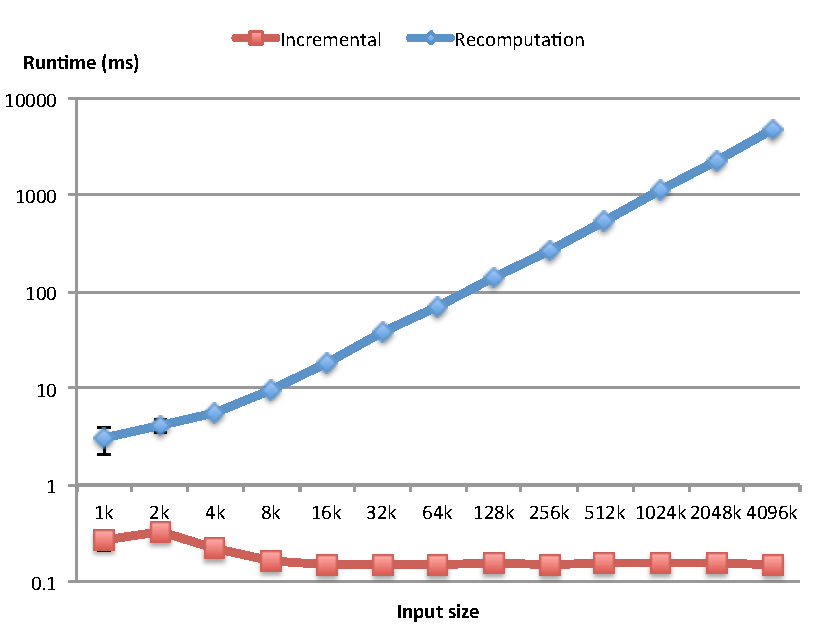
\includegraphics[keepaspectratio,width=8.5cm]{pldi14/HistogramGenerated-new.pdf}
\caption{Performance results in log-log scale, with input size on
  the x-axis and runtime in ms on the y-axis. Confidence
  intervals are shown by the whiskers; most whiskers are
  too small to be visible.}
\label{fig:graph}
\end{figure}
